\documentclass{article}
\usepackage[italian]{babel}
\usepackage[tmargin=2cm,rmargin=1.5in,lmargin=1.5in,margin=0.85in,bmargin=2cm,footskip=.2in]{geometry}
\usepackage{siunitx}
\sisetup{separate-uncertainty=true, per-mode=fraction, parse-numbers=true}
\usepackage{caption}
\usepackage[T1]{fontenc}
\usepackage{bookmark}
\usepackage{mathcomp}
\usepackage{graphicx}
\usepackage{multicol}
\usepackage{booktabs}
\usepackage{amsmath,amsfonts,amsthm,amssymb,mathtools}
\hypersetup{
	pdftitle={Relazione conducibilità termica},
	colorlinks=true, linkcolor=doc!90,
	bookmarksnumbered=true,
	bookmarksopen=true
}
\usepackage{blindtext}
\usepackage{wrapfig}
\usepackage{listings}
\usepackage{xcolor}
\usepackage{float}
\usepackage{tikz}
\usepackage{multirow}
\usepackage{biblatex}
\definecolor{codegreen}{rgb}{0,0.6,0}
\definecolor{codegray}{rgb}{0.5,0.5,0.5}
\definecolor{codepurple}{rgb}{0.58,0,0.82}
\definecolor{backcolour}{rgb}{0.95,0.95,0.92}
\definecolor{doc}{rgb}{0,0,0}
\lstdefinestyle{code}{
    backgroundcolor=\color{backcolour},   
    commentstyle=\color{codegreen},
    keywordstyle=\color{magenta},
    numberstyle=\tiny\color{codegray},
    stringstyle=\color{codepurple},
    basicstyle=\ttfamily\footnotesize,
    breakatwhitespace=false,         
    breaklines=true,                 
    captionpos=b,                    
    keepspaces=true,                                     
    showspaces=false,                
    showstringspaces=false,
    showtabs=false,                  
    tabsize=2,
    inputencoding=ansinew,
    extendedchars=true,
    numbers=left,                    
    numbersep=5pt
}

\lstset{style=code}
\usepackage[varbb]{newpxmath}
\usepackage{circuitikz}
\captionsetup{labelfont={bf, sc}}

\title{Relazione oscillazioni accopiata}
\author{Aiello Giosuè, Fenili Domenico, Sermi Francesco}
\date{\today}

\begin{document}
\maketitle
\newpage
\tableofcontents

\newpage
\section{Scopo}
Studiare il moto di due pendoli accoppiati e del fenomeno dei \emph{battimenti}
\section{Premesse teoriche}
Dato un pendolo fisico, sappiamo che il suo moto può essere determinato risolvendo la seguente equazione del moto:
\begin{equation}
	-mg\sin{\theta} = \frac{d\vec{L}}{dt} = I\frac{d^2 \theta}{dt^2}
\end{equation}
da cui possiamo ricavare, nell'ipotesi delle piccole oscillazioni attorno al punto di equilibrio, la pulsazione del pendolo, pari a
\begin{equation}
	\omega_0 = \sqrt{\frac{mgd}{I}}
\end{equation}
dove $d$ rappresenta la distanza del perno dal centro di massa dell'oggetto, mentre $I$ il momento di inerzia del corpo. \\
Nel caso delle oscillazioni accoppiate, esistono una serie di modi, detti \emph{normali}, con cui è possibile far oscillare il corpo: il primo modo consiste nel far partire i due pendoli con la stessa ampiezza spostandoli nello stesso \emph{verso} e lasciandoli andare nello stesso momento: in questo caso la molla, utilizzata per accoppiare le due oscillazioni, non sarà sollecitata e non andrà ad influenzare il moto dei due pendoli, i quali oscilleranno sincroni alla frequenza posseduta quando oscillano \emph{singolarmente}. L'altro modo, invece, si ha spostando i pendoli in versi opposti ma con la stessa ampiezza e, in questo caso, la molla sollecitata andrà invece ad influenzare il moto.
\section{Descrizione delle misure}

Per effettuare questa esperienza era necessario misurare il periodo di oscillazione delle oscillazioni accoppiate in varie situazioni. \\
Prima di procedere però con le misurazioni di questi, abbiamo misurato la lunghezza dell'asta che oscillava e la sua larghezza, che risulta essere pari a
\begin{align*}
    &L = & &
\end{align*}
e abbiamo misurato il raggio e lo spessore del disco a cui l'asta era attaccata, pari a
\begin{align*}
    &R = & & 
\end{align*}
\begin{minipage}{0.5\textwidth}
    \centering
    \begin{tabular}{c c c c}
        \toprule
        Tempo A & Posizione A & Tempo B & Posizione B \\
        $(s)$ &  $u.a.$ & $s$ & $u.a.$ \\ \toprule
        0.026 & 504 & 0.051 & 233 \\
        0.076 & 504 & 0.101 & 282 \\
        0.127 & 505 & 0.153 & 365 \\
        0.177 & 503 & 0.203 & 424 \\
        0.228 & 502 & 0.254 & 478 \\
        0.279 & 503 & 0.304 & 541 \\
        0.330 & 504 & 0.355 & 602 \\
        0.381 & 503 & 0.406 & 657 \\ \bottomrule
    \end{tabular}
    \captionsetup{format=plain}
    \captionof{table}{Misure registrare dal PC tramite il programma di registrazione \emph{plasduino}: il \texttt{Tempo A} è il tempo in cui avveniva il campionamento del pendolo $A$ mentre \texttt{Posizione A} la rispettiva posizione del pendolo in quegli istanti di tempo. Quanto detto vale per il pendolo $B$ riguardo \texttt{Tempo B} e \texttt{Posizione B}}
\end{minipage}
\hspace{0.01\textwidth}
\begin{minipage}{0.49\textwidth}
Dopo aver effettuato questo, abbiamo iniziato a misurare l'oscillazione del singolo pendolo prima senza lo smorzatore e poi senza lo smorzatore: ai fini di queste misure, abbiamo usufruito di un programma di acquisizione che girava sul PC che avevamo a disposizione in laboratorio che andava a stimare la posizione del pendolo in $u.a$ (unità arbitrarie) in base alla variazione di corrente dovuta al passaggio del pendolo nell'acqua lì presente. \\
Dopo aver effettuato queste misure, siamo passati ad analizzare il moto del pendolo se accoppiato ad un altro pendolo facendoli oscillare secondo i modi normali dell'oscillazione: per fare ciò abbiamo utilizzato una molla con cui abbiamo collegato i due pendoli e, successivamente, li abbiamo fatti oscillare prima facendoli partire alla stessa ampiezza e poi facendoli partire da ampiezza opposta (in verso). \\
Infine, abbiamo misurato le oscillazioni compiuti da un pendolo messo in movimento ma accoppiato ad un altro che parte da fermo. \\
Riporto qua di lato un esempio di misurazione eseguita dal PC.
\end{minipage}
Per calcolare i periodi delle varie oscillazioni abbiamo creato un programma in Python in grado di effettuare uno \emph{smoothing} delle misure per poi utilizzare la libreria \texttt{find\_peaks} per trovare i massimi relativi. I periodi delle oscillazioni a quel punto sono stati calcolati prendendo la differenza fra due massimi consecutivi, tuttavia rimandiamo all'appendice per una trattazione più esaustiva del processo.

\section{Analisi delle misure}

In primis siamo andati a calcolare il momento di inerzia del nostro pendolo fisico: per fare ciò dovevamo calcolare la posizione del centro di massa del nostro corpo e la massa. \\
\textbf{Osservazioni}: sebbene l'asta presentasse dei \emph{buchi}, abbiamo considerato come trascurabile lo spostamento del centro di massa dovuto a questi. Oltre a ciò l'asta e il disco si sono considerati omogenei, quindi la loro densità era costante in ogni punto del materiale, e nel calcolo del momento di inerzia abbiamo considerato la sbarra come un'asta con spessore trascurabile rispetto al dimensioni effettive del calcolo. \\
Per calcolare il momento di inerzia siamo quindi andati a calcolare la massa del disco di ottone e la massa dell'asta usando la densità dei due materiali
\begin{align*}
	&m_O = \rho_O V_O = \rho_o \pi r^2 d \approx & &m_A = \rho_A V_A = \rho_A Llh \\
	&\sigma_O = m_0 \sqrt{4 \left(\frac{\sigma_r}{r} \right)^2 + \left( \frac{\sigma_d}{d} \right)^2}  & &\sigma_A = m_A \sqrt{ \left(\frac{\sigma_L}{L} \right)^2 + \left( \frac{\sigma_l}{l} \right)^2 + \left( \frac{\sigma_h}{h} \right)^2}
\end{align*}
mentre per calcolare il momento di inerzia possiamo usare il teorema di Hyugens-Steiner
\begin{align*}
	I_P = I_{CM} + Md^2
\end{align*}
Ora, la nostra strumentazione può essere schematizzata nella seguente maniera:
\begin{figure}[H]
	\centering
\begin{tikzpicture}[scale=1.5, rotate=-36.25]

% Disegno dell'asta
\draw[thick] (0,0) -- (3,0);
\filldraw (0,0) circle (2pt);
\filldraw (3,0) circle (2pt);

% Disegno del cilindro
\draw[thick] (3,0) circle (0.5);
\filldraw (3,0) circle (2pt);

% Linea tratteggiata per indicare l'ampiezza
\draw[dashed] (0,0) -- (1.5,-2) node[midway, left] {$l$};

% Etichetta per l'asta
\node at (1.5,0.3) {$L$};

% Etichetta per il cilindro
\node at (3.7,0) {$m$};

% Etichetta per l'ampiezza
\node at (0.75,-2) {$A$};

% Etichetta per l'angolo
\draw (0.5,0) arc (0:-50:0.5);
\node at (0.6,-0.2) {$\theta$};

\end{tikzpicture}
\caption{Schematizzazione del nostro apparato sperimentale, costituito da un'asta il cui spessore può essere trascurato rispetto alla lunghezza $L$}
\end{figure}
quindi possiamo calcolarci il momento di inerzia di questo corpo considerandolo come l'unione di un'asta rigida e un disco di spessore non trascurabile, dunque il momento di inerzia delle sue "parti" risulta essere pari a:
\begin{align*}
	&I_C = \frac{1}{12} M_C R^2_C & &I_A = \frac{M_A L^2}{3} + 
\end{align*}
%Ci siamo calcolati la pulsazione del moto armonico del pendolo realizzando anche un programma in Python che analizzava le misurazioni fatte dal PC effettuando prima uno \emph{smooth} della nostra funzione tramite una \emph{spline} (grazie alle funzionalità della libreria \texttt{scipy.interpolate}) e poi, grazie alla funzione \texttt{find\_peaks} della libreria \texttt{scipy.signal}, ci trovava i massimi di questa curva. A quel punto, 
Per misurare la pulsazione, bastava considerare la distanza di tempo fra due massimi consecutivi. Sebbene avessimo effettuato un'operazione di \emph{smoothing} della curva che introduceva dei nuovi punti \emph{virtuali}, l'errore che si commetteva considerando i nuovi massimi non influiva di molto sulla misura del tempo, siccome la funzione \texttt{CubicSpline}, se ritiene che si trovi fra due punti \emph{reali} va ad inserire il massimo nel punto medio compreso fra i due punti (eventualmente modificando i punti precedenti per \emph{accordare} lo smoothing). Pertanto, visto che eravamo interessati solamente al tempo e non al valore delle ampiezze, l'errore che si commetteva considerando due massimi \emph{virtuali}, ovvero inseriti dal programma, era trascurabile, siccome il computer campionava sempre dopo un intervallo di tempo di circa $0.5 \, s$ dunque lo spline andava a spostarli sempre di un intervallo costante che si cancellava nel momento in cui si consideravano le ascisse di due massimi consecutivi. \\
Ci siamo calcolati, per ogni massimo individuato dalla funzione \texttt{find\_peaks}, la distanza temporale fra i due massimi e abbiamo effettuato la media aritmetica dei tempi trovati:
\begin{equation}
	T = \frac{\sum\limits_{i=1}^{n+1} t^{*}_{i+1} - t^{*}_i}{n}
\end{equation}
dove con $t^{*}_{i}$ indicavamo la posizione dell'$i$-esimo massimo e come errore sulla media abbiamo utilizzato la deviazione standard della media aritmetica
\begin{equation}
	\sigma_{T} = \sqrt{\frac{1}{n(n-1)}\sum_{k=1}^{n}{T_k}}
\end{equation}
riportiamo la misura di tutti i periodi nei varie casistiche in cui abbiamo studiato il fenomeno nella tabella della prossima pagina.

\begin{table}
\centering
\begin{tabular}{l c c} \toprule
Descrizione & Media dei periodi ($\si{\second}$) & Pulsazione ($\si{\radian\per\second}$) \\ \\ \toprule
Oscillazioni senza smorzatore & $1.415 \pm 0.003$ & $4.440 \pm 0.008$ \\ \midrule
Oscillazioni con smorzatore & $1.38 \pm 0.04$ & $4.5 \pm 0.1$ \\ \midrule
Oscillazioni accoppiate in fase & $1.413 \pm 0.001$ & $4.444 \pm 0.004$ \\ \midrule
Oscillazioni accoppiate in controfase & $0.88 \pm 0.2$ & $7 \pm 1$ \\ \bottomrule
\end{tabular}
\captionof{table}{Tabella con le misure da noi effettuate, riportiamo a sinistra la descrizione in breve del tipo di fenomeno studiato, nella tabella centrale la media dei valori dei periodi ottenuti facendo la distanza temporale fra due massimi consecutivi e, infine, la pulsazione $\omega_0$ calcolata nei vari casi: come possiamo vedere l'errore che abbiamo sulle oscillazioni in controfase e nelle oscillazioni con smorzatore dovuto al fatto che abbiamo effettuato delle misure in cui abbiamo fatto partire i due pendoli non allo stesso momento e questo stacco fra i due non è trascurabile mentre nelle oscillazioni con smorzatore il motivo probabilmente è dovuto al fatto che la pallina è stata influenzata troppo dagli attriti del fluido alle estremità del bordo}
\end{table}

\noindent Per calcolare la pulsazione $\omega_0$, sempre riportata nella tabella di fianco, abbiamo utilizzato la seguente relazione:
\begin{equation}
	\omega_0 = \frac{2\pi}{T}
\end{equation}
dove $T$ è la media dei periodi. Come errore, abbiamo considerato il fatto che gli errori relativi statici si conservano durante prodotti e divisioni, dunque:
\begin{equation*}
	\frac{\sigma_{\omega_0}}{\omega_0} = \frac{\sigma_{T}}{T} \, \implies \, \sigma_{\omega_0} = \frac{\sigma_T}{T} \omega_0 = \frac{\sigma_T}{T} \frac{2\pi}{T} = \frac{2\pi \sigma_T}{T^2}
\end{equation*}
Abbiamo anche stimato il tempo di decadimento dell'ampiezza del moto con smorzatore tramite il metodo del parametro libero tramite fit: abbiamo usato come modello teorico per le nostre misure il seguente
\begin{equation}
	x(t) = \theta_0 (0)e^{-\frac{t}{\tau}}\cos{\left( \omega t + \phi \right) }
	\label{eq:modello_teorico}
\end{equation}
Sebbene le ampiezze massima dell'oscillazione variava, in funzione del tempo, nella seguente maniera
$$
	\theta_0 (t) = \theta_0 (0) e^{-\frac{t}{\tau}}
$$
abbiamo deciso di utilizzare il modello descritto dalla \ref{eq:modello_teorico} siccome non riuscivamo a stimare qual era l'errore che si commetteva considerando come massimo una misurazione da noi compiuta oppure prendendo come massimo una misurazione \emph{virtuale}, ovvero un massimo aggiunto dall'operazione di smoothing della curva. In questa maniera, ad ogni punto potevamo assegnare come incertezza quella strumentale, pari a $1 \, u.a$ (si poteva anche pensare che lo strumento, in quanto digitale, seguisse una distribuzione uniforme, dunque l'errore sarebbe pari a $\frac{1}{\sqrt{12}}$ ma abbiamo ritenuto che l'errore effettivo, che già è piccolo, fosse sottostimato di troppo oltre al fatto che andremo a sottostimare la risoluzione strumentale dello strumento utilizzato). \\
Riportiamo il grafico del fit:

\begin{wrapfigure}{r}{0.3\textwidth}
	\centering
	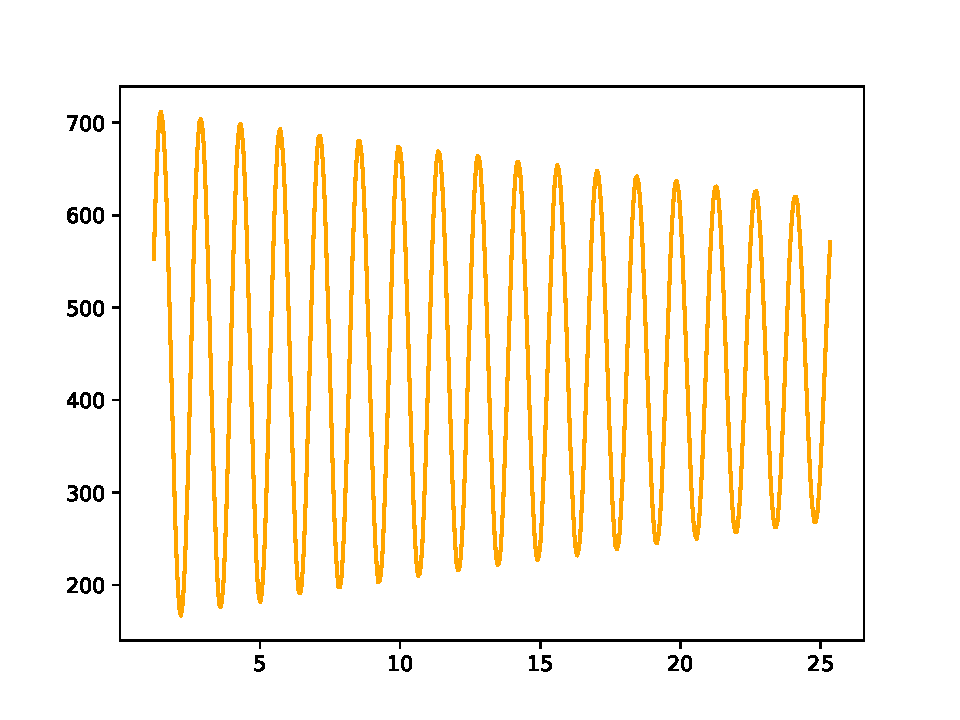
\includegraphics[scale=0.6]{Grafico_oscillazione_accoppiate_senza_smorzatore.pdf}
\end{wrapfigure}


\end{document}